\documentclass[a4paper,11pt]{article}
\usepackage[T1]{fontenc}
\usepackage[utf8]{inputenc}
\usepackage{lmodern}

\usepackage{amsmath}
\usepackage{amsthm}

\usepackage{graphicx}
\graphicspath{{../data/}}
\usepackage{caption}

\usepackage{fullpage}

\renewcommand{\thesubsection}{\alph{subsection}}

\newcommand{\pitem}[2]{
\item
\begin{tabular*}{3in}{p{1in}p{1.2in}}
		#1 & \hfill #2 \\
\end{tabular*}\vspace{-6pt}}

\title{Image Processing 1 - Exercise 7 - WiSe 2012/13}
\author{Weipeng He \\ \texttt{2he@informatik.uni-hamburg.de} \\ \texttt{6411529}}

\begin{document}

\maketitle

\section{Preprocessing}

Read the color image, convert to grayscale, normalize to $[0.0, 1.0]$. Then use threshold ($0.68$) to make the image black and white, in order to remove the noise. The preprocessed image is shown below :
\begin{center}
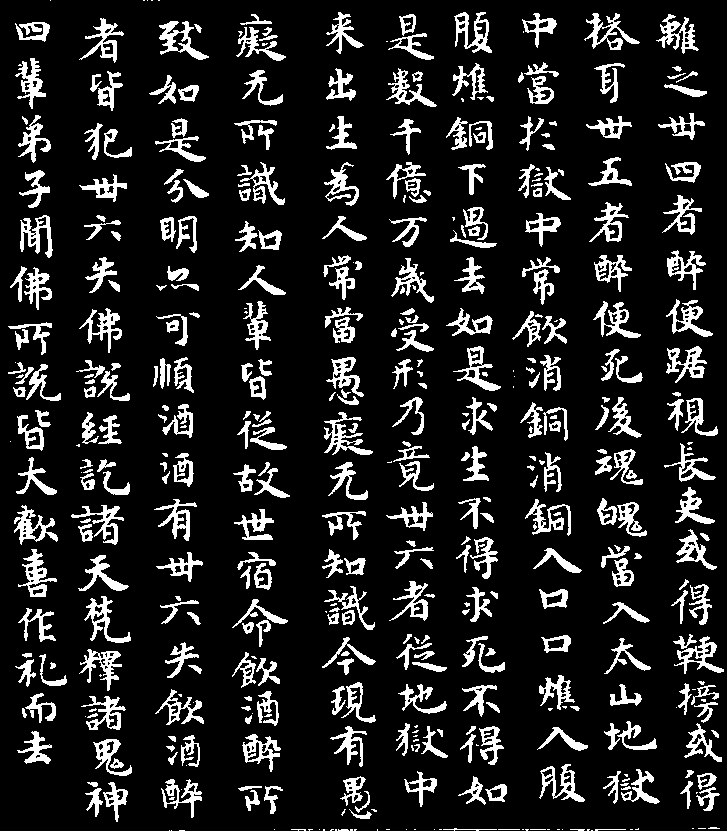
\includegraphics[width=.8\textwidth]{preproc}
\end{center}

\section{Finding candidates characters}

Filter the image using a convolution mask shown below:
\[
 \begin{pmatrix}
  -2 & -2 & -2 & -2 & \cdots & -2 & \cdots & -2 & \cdots & -2 \\
  -2 & -1 & -1 & -1 & \cdots & -1 & \cdots & -1 & \cdots & -2 \\
  -2 & -1 & 0 & 0 & \cdots & 0 & \cdots & 0 & \cdots & -2 \\
  -2 & -1 & 0 & 1 & \cdots & 1 & \cdots & 1 & \cdots & -2 \\
  \vdots & \vdots & \vdots & \vdots & \ddots & \vdots & \ddots & \vdots & \ddots & -2 \\
  -2 & -1 & 0 & 1 & \cdots & 5 & \cdots & 5 & \cdots & -2 \\
  \vdots & \vdots & \vdots & \vdots & \ddots & \vdots & \ddots & \vdots & \ddots & -2 \\
  -2 & -1 & 0 & 1 & \cdots & 5 & \cdots & 5 & \cdots & -2 \\
  \vdots & \vdots & \vdots & \vdots & \ddots & \vdots & \ddots & \vdots & \ddots & -2 \\
  -2 & -2 & -2 & -2 & \cdots & -2 & -2 & -2 & \cdots & -2 \\
 \end{pmatrix}
\]
The size of the mask is about the same with an average character ($51 \times 51$), the value of the center is high (maximum of $5$) and the margin is negative. The mask can detect where are likely to be a character.

Afterwards, use maximum filter to find out local maximum which are not less than all neighbor pixels(distance less than $30$). From these points, I find the best fit box which make the density of 3-pixel margin to be low ($0.05$). Then, the candidate characters are found. Results are shown below:
\begin{center}
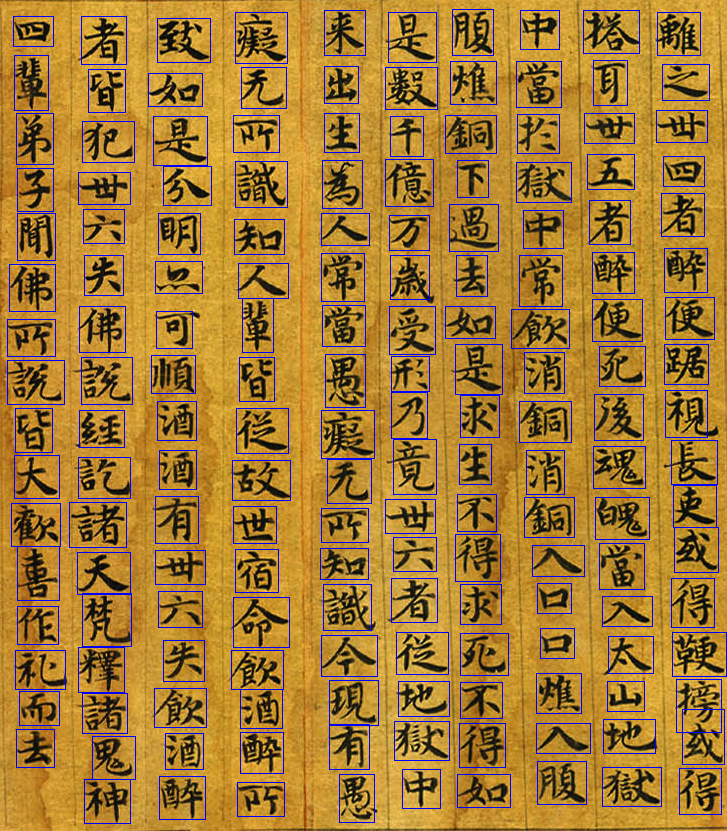
\includegraphics[width=.8\textwidth]{cand}
\end{center}

\clearpage
\section{Finding Points of Interest}
I calculate the points of interest using standard SIFT algorithm, which is caculating the DoG pyramid.

\section{Generating SIFT-Features}
I calculate the feature descriptor using standard SIFT algorithm. 

\section{Retrieval}
The retrieval of matching character is done by comparing the template and the candidate character (subpicture of the original) one by one. A quality score is given for classifying if these two charater match.

First, I use brute force matching to find out nearest neighbor of each key points in the template. Then, calculate the score of each match by :
\[
  Score = \frac{1.0}{.1 + Distance^2}
\]
where the $Distance$ is the matching distance. Divide scores by the maximum score, so that the maximum score is $1.0$. Filter out the matches with score less than $0.4 \times MaxScore$.

For each match, I can calulate the shifts in x and y direction (denote by array $ShiftX$ and $ShiftY$). The quality score is the weighted standard deviation (using score as weight) of the shifts.
\[
  Quality = \sqrt{\frac{\sum_{i=1}^{n} Score_i ((ShiftX_i-\bar{ShiftX})^2 + (ShiftY_i-\bar{ShiftX})^2)} {\sum_{i=1}^{n} Score_i - 1.0}}
\]
Those pair of candidate and template with quality score less than $2.0$ is considered to be matched. And, the mean of shifts in x and y can be used to calculate the match position.

\clearpage
\section{Results}
\subsection{}
Template:
\begin{center}

\includegraphics[width=.2\textwidth]{test1}
\end{center}
Result:
\begin{center}
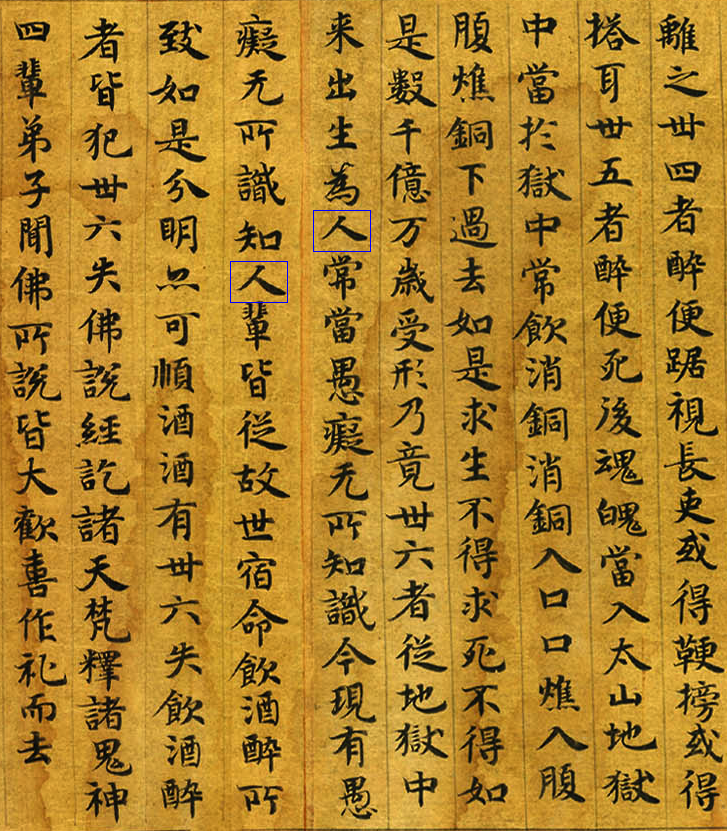
\includegraphics[width=.8\textwidth]{result1}
\end{center}

\clearpage
\subsection{}
Template:
\begin{center}
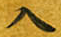
\includegraphics[width=.2\textwidth]{test2}
\end{center}
Result:
\begin{center}
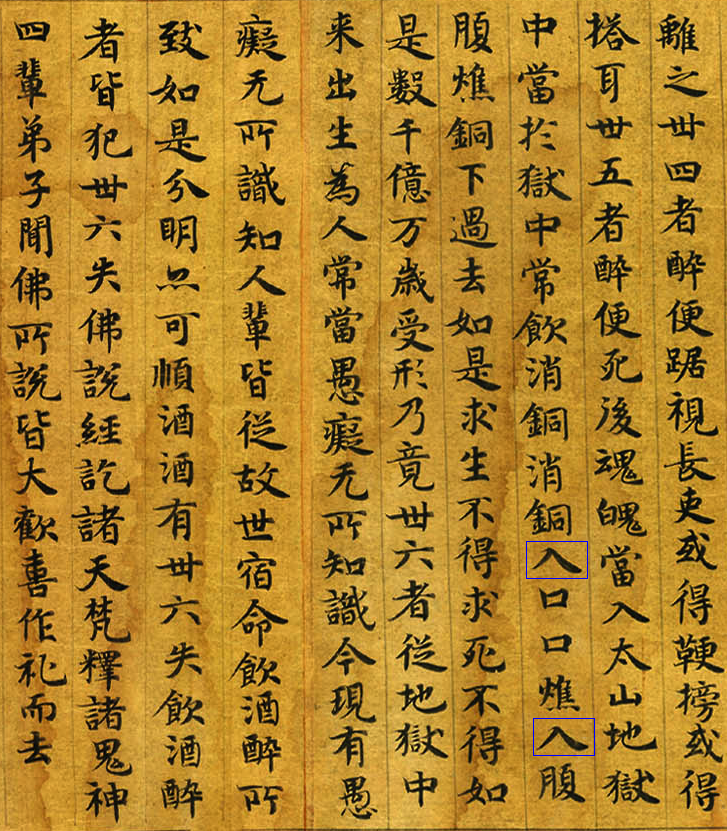
\includegraphics[width=.8\textwidth]{result2}
\end{center}

\clearpage
\subsection{}
Template:
\begin{center}

\includegraphics[width=.2\textwidth]{test6}
\end{center}
Result:
\begin{center}
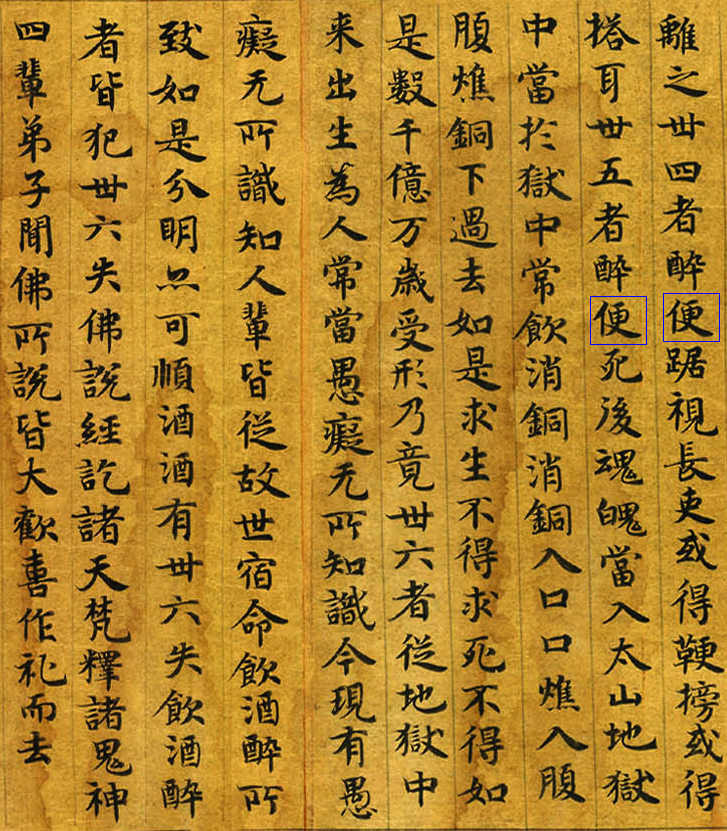
\includegraphics[width=.8\textwidth]{result6}
\end{center}

\clearpage
\subsection{}
Template:
\begin{center}

\includegraphics[width=.2\textwidth]{test4}
\end{center}
Result:
\begin{center}
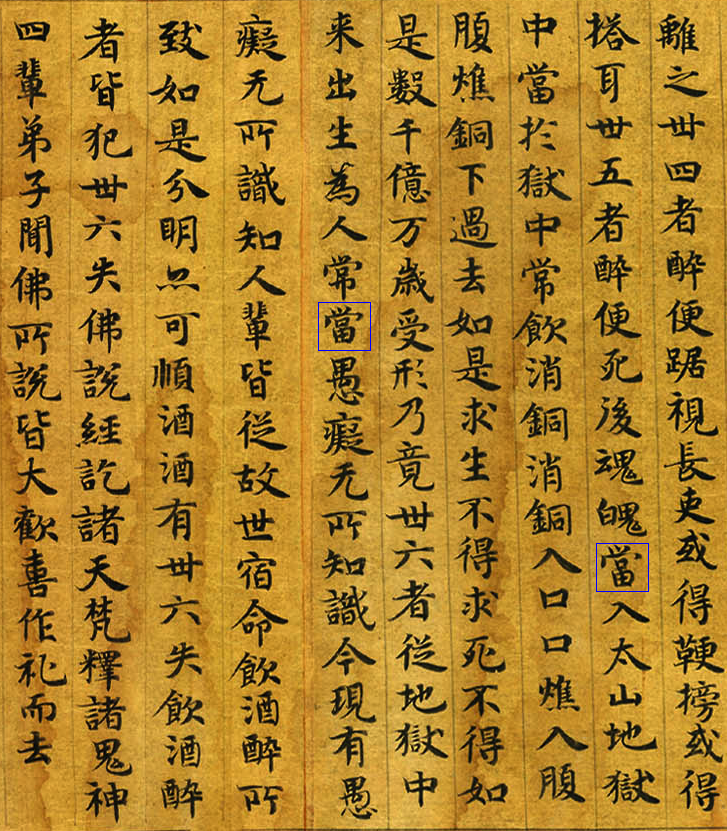
\includegraphics[width=.8\textwidth]{result4}
\end{center}

\end{document}
